\documentclass[11pt]{article}

\usepackage[utf8]{inputenc}
% ============================================================
% SHARED PREAMBLE -- included by Internship_Report_EN.tex and
% Rapport_de_Stage_FR.tex. Keeps both language versions visually
% identical. Edit style here, not in the two content files.
% ============================================================

\usepackage[T1]{fontenc}
\usepackage[margin=1in]{geometry}
\usepackage{graphicx}
\graphicspath{{../plots/}{./figures/}}

\usepackage{amsmath}
\usepackage{amssymb}

\usepackage{booktabs}
\usepackage{array}
\usepackage{tabularx}
\usepackage{adjustbox}
\usepackage{caption}
\usepackage[table]{xcolor}
\usepackage{enumitem}

\usepackage{tikz}
\usetikzlibrary{arrows.meta, positioning}

\usepackage{fancyhdr}
\usepackage{titlesec}

% ------------------------------------------------------------
% COLOR
% ------------------------------------------------------------
\definecolor{umorange}{RGB}{215,74,42}

% ------------------------------------------------------------
% TABLE DEFAULTS
% ------------------------------------------------------------
\AtBeginEnvironment{table}{\centering}
\captionsetup[table]{justification=centering, singlelinecheck=false}
\captionsetup[figure]{justification=centering, singlelinecheck=false}
\renewcommand{\arraystretch}{1.2}
\newcolumntype{Y}{>{\centering\arraybackslash}X}

% Light rule usable inside tabular/tabularx bodies between rows
\newcommand{\rowrule}{\midrule[0.2pt]}

% ------------------------------------------------------------
% HEADER / FOOTER
% ------------------------------------------------------------
\newcommand{\ReportHeaderLeft}{}
\newcommand{\ReportHeaderRight}{}

\pagestyle{fancy}
\fancyhf{}
\renewcommand{\headrulewidth}{0.4pt}
\renewcommand{\footrulewidth}{0pt}
\fancyhead[L]{\slshape\small\ReportHeaderLeft}
\fancyhead[R]{\slshape\small\ReportHeaderRight}
\fancyfoot[C]{\thepage}

\fancypagestyle{plain}{
  \fancyhf{}
  \fancyfoot[C]{\thepage}
  \renewcommand{\headrulewidth}{0pt}
  \renewcommand{\footrulewidth}{0pt}
}

% ------------------------------------------------------------
% SECTION / SUBSECTION STYLE -- bold title + thin orange rule
% ------------------------------------------------------------
\titleformat{\section}
  {\Large\bfseries}
  {\thesection}
  {0.6em}
  {}
  [{\color{umorange}\titlerule[1pt]}]
\titlespacing*{\section}{0pt}{3.2ex plus 1ex minus .2ex}{1.6ex plus .2ex}

\titleformat{\subsection}
  {\large\bfseries}
  {\thesubsection}
  {0.6em}
  {}
\titlespacing*{\subsection}{0pt}{2.6ex plus 1ex minus .2ex}{1ex plus .2ex}

\titleformat{\subsubsection}
  {\bfseries}
  {\thesubsubsection}
  {0.6em}
  {}
\titlespacing*{\subsubsection}{0pt}{2ex plus 1ex minus .2ex}{0.8ex plus .2ex}

% ------------------------------------------------------------
% TIKZ NODE STYLE -- shared by every pipeline/workflow diagram
% ------------------------------------------------------------
\tikzset{
  rbox/.style={draw, rounded corners, fill=umorange!12, align=center,
               minimum height=1.05cm, text width=#1, font=\small},
  rbox/.default=2.6cm,
  flow/.style={-{Latex[length=2.2mm]}, thick}
}


\newcommand{\ReportTitleShort}{Internship Report -- ML-Augmented Shock-Capturing Schemes}
\renewcommand{\ReportHeaderLeft}{\ReportTitleShort}
\renewcommand{\ReportHeaderRight}{Yasser Baouzil}

\begin{document}

% ============================================================
% TITLE PAGE
% ============================================================
\begin{titlepage}
\thispagestyle{empty}

\begin{center}

\includegraphics[width=0.55\textwidth]{um6p_college_of_computing_logo.png}
\end{center}

\vspace{4.5cm}

\begin{center}
{\Huge\bfseries Internship Report}\\[1.2cm]
{\Large Machine-Learning-Augmented Shock-Capturing Schemes for\\
Conservation Laws: From Imitation Learning to an\\
Unrolled Physics Loss}\\[0.4cm]
{\large UM6P -- College of Computing}
\end{center}

\vspace{3cm}

\begin{center}
\begin{tabular}{ll}
\textbf{Student} & Yasser Baouzil \\
\textbf{Host institution} & UM6P -- College of Computing \\
\textbf{Internship tutor} & Radouan Boukharfane \\
\textbf{Academic supervisor} & Radouan Boukharfane \\
\textbf{Period} & From 01/06/2026 to 01/08/2026 \\
\textbf{Duration} & 2 months \\
\textbf{Level} & First year of the engineering cycle \\
\end{tabular}
\end{center}

\vfill

\begin{center}
\color{umorange}\rule{0.5\textwidth}{0.6pt}
\end{center}

\begin{center}
Academic year 2025-2026
\end{center}

\end{titlepage}

% ============================================================
% CONTENTS
% ============================================================
\tableofcontents
\thispagestyle{plain}
\newpage

% ============================================================
\section{Abstract}

This report presents the work carried out during a two-month internship at
UM6P -- College of Computing, under the supervision of Radouan Boukharfane.
The project studies whether a neural network can improve on classical
shock-capturing finite-volume schemes (WENO5, TENO5) for hyperbolic
conservation laws, and, more importantly, whether the way such a network is
\emph{trained} determines what kind of improvement is even possible.

The work is built in two layers. The first layer reproduces and extends an
existing result from the literature: a network trained by \emph{imitation}
to reproduce a classical scheme's own reconstruction decision, evaluated
against that same classical scheme on scalar advection, Burgers' equation,
and the Euler system (Sod shock tube, Shu--Osher problem). By construction,
an imitation-trained network can never systematically exceed the quality of
the scheme it imitates -- and the measurements confirm this directly.

The second, larger layer tests an alternative proposed by the internship
supervisor: an \emph{Unrolled Physics Loss}. Instead of imitating a
classical scheme's decision one stencil at a time, the network is trained
by running it through several actual simulation steps and judging the
resulting trajectory against the real solution. This required a
from-scratch, fully differentiable JAX reimplementation of the project's
numerical core, since nothing in the original NumPy/Keras codebase is
differentiable end-to-end.

The Unrolled Physics Loss produces the project's only genuine, verified
wins against the classical scheme: on the scalar Burgers and advection
benchmarks, and on the Euler Shu--Osher problem. It also exposes a real,
diagnosed numerical-stability failure mode on the Euler system, traced to
Roe-eigenbasis conditioning under an evolving network reconstruction, and a
genuine structural ceiling on the Sod shock tube that further tuning cannot
cross. Both positive and negative results are reported with the same level
of detail, because the value of this internship is in what was learned
about \emph{why} each approach does or does not work, not only in the
final numbers.

% ============================================================
\section{Introduction}

Shock-capturing schemes such as WENO (Weighted Essentially Non-Oscillatory)
and TENO (Targeted Essentially Non-Oscillatory) are the numerical backbone
of high-fidelity compressible-flow simulation. They reconstruct a smooth,
high-order interpolant everywhere except across a discontinuity, where they
fall back to a lower-order, non-oscillatory one. The rule that decides
\emph{where} to fall back is itself hand-designed: a smoothness indicator,
compared against a threshold, computed independently at every cell
interface.

Replacing that hand-designed rule with a trained neural network is an
appealing idea: a network can in principle learn a decision boundary more
finely tuned to the data than a fixed analytic formula. The published
WENO5-NN result (Stevens \& Colonius, 2020) shows this is possible for a
WENO5 scheme. This internship first reproduces that result, then asks a
harder question: can the same idea be pushed further for TENO5 -- and, more
fundamentally, does \emph{how} the network is trained change what kind of
improvement is achievable at all?

The report is organized to answer that question in the order it was
actually investigated: numerical background, the original imitation-based
approach and its structural ceiling, the Unrolled Physics Loss proposed as
an alternative, the differentiable infrastructure it required, and the
results and failure modes it produced on both scalar and system (Euler)
problems.

% ============================================================
\section{Internship Context}

The internship took place at UM6P -- College of Computing, over two months
(June--August 2026), supervised by Radouan Boukharfane, who also proposed
the internship's central research question and its second phase (the
Unrolled Physics Loss). The subject, as stated on the internship's own
technical sheet, was \emph{``Machine learning-based numerical scheme for
CFD''}, with three stated missions: a literature review, building a neural
network to compute the weighting functions used inside a WENO-family
scheme, and assessing its performance.

The internship builds directly on top of an existing open-source codebase
implementing the original WENO5-NN paper. Rather than starting from a blank
page, the work extends that codebase to TENO5, reproduces its published
claims as a baseline, and then tests a training methodology the published
work does not use.

Because the subject is a research question rather than a fixed
specification, the work was organized as a sequence of falsifiable
experiments rather than a single linear implementation plan: each phase
proposes a specific mechanism, tests it against the real solution, and
either keeps it, fixes it, or discards it based on the measured outcome.
This experimental discipline is reflected directly in the results reported
later in this document.

% ============================================================
\section{Project Objectives, Scope, and Missions}

The internship's objective was to determine whether a neural network can
improve on TENO5, a state-of-the-art classical shock-capturing scheme, and
to do so with results that are measured against the true solution rather
than against the classical scheme's own output.

The three missions defined at the start of the internship were:

\begin{itemize}
    \item \textbf{Bibliography}: survey the literature on machine-learning
    augmented WENO/TENO schemes, and on the Boundary Variation Diminishing
    (BVD) principle used later in the loss function.
    \item \textbf{Neural network}: build a network that computes the
    weighting/selection function inside a WENO-family reconstruction
    (which candidate stencil to trust at each interface).
    \item \textbf{Assessment of performance}: measure that network's
    accuracy against the classical scheme it augments, on canonical test
    problems, not only on held-out training data.
\end{itemize}

The scope was intentionally kept to fifth-order schemes (WENO5, TENO5) on
one-dimensional scalar and Euler test problems: linear advection, Burgers'
equation, the Sod shock tube, and the Shu--Osher problem. Higher orders
(WENO3/WENO7, TENO3/TENO7) and multi-dimensional problems exist as
reconstruction modules in the codebase but were explicitly left out of the
neural-network training scope, since no order-3 or order-7 training dataset
exists and building one was not part of the stated missions.

A fourth, unplanned objective emerged directly from the first two months of
work: once it became clear that imitation training has a structural ceiling
(Section~\ref{sec:strand2}), the internship's scope grew to include
designing, implementing, and evaluating an alternative training paradigm --
the Unrolled Physics Loss -- proposed by the academic supervisor
specifically to remove that ceiling.

% ============================================================
\section{Work Methodology}

The project was organized as a chronological sequence of numbered
experiments (21 in total by the end of the internship), each with a stated
goal, a concrete falsification criterion, and a documented outcome --
whether positive, negative, or partial. This discipline was adopted early,
after an initial (uninstrumented) attempt made it difficult to tell whether
an apparent improvement was real or an artifact of how it was measured.

Two evaluation criteria were used throughout, applied consistently to
every experiment:

\begin{itemize}
    \item \texttt{beats\_teacher}: the network's error against the
    \emph{true} solution is strictly lower than the classical scheme's
    error against the true solution. This is the criterion used for every
    claim of a ``win'' in this report.
    \item \texttt{teacher\_fidelity}: the network's error is within a
    small margin (2\%) of the classical scheme's error. This looser
    criterion was only used for early acceptance tests and is never used to
    claim superiority.
\end{itemize}

Each experiment was run, measured against both criteria on canonical
(non-training) benchmarks, and documented immediately -- including
experiments that made things worse. This is why the project's internal
experiment log (\texttt{Documentation/Results.md}) records 21 phases rather
than a handful of curated successes: several fixes that seemed correct on
paper (Section~\ref{sec:instability}) measurably failed and had to be
reverted or replaced.

A second methodological choice, adopted after losing a working checkpoint
to an un-backed-up experiment, was to commit and back up every verified
good result immediately, before starting the next experiment on top of it.

% ============================================================
\section{Scientific Background: Finite-Volume Methods for Conservation Laws}
\label{sec:background-fv}

A scalar hyperbolic conservation law,
\[
\partial_t u + \partial_x f(u) = 0,
\]
and the compressible Euler system (its vector generalization, with $u$ the
vector of conserved density, momentum, and energy, and $f(u)$ the
corresponding physical flux) are both solved here with the method of lines:
the spatial domain is divided into $N$ cells, each cell $i$ stores a
cell-average $u_i$, and the equation is advanced by estimating the flux at
every cell interface $i+1/2$ and integrating
\[
\frac{d u_i}{dt} = -\frac{1}{\Delta x}\left(\hat f_{i+1/2} - \hat f_{i-1/2}\right)
\]
in time with an explicit Runge--Kutta scheme. Throughout this project this
is third-order SSPRK3 (Shu \& Osher's strong-stability-preserving form,
used identically in Stevens \& Colonius' own paper), chosen because each of
its stages is itself a convex combination of forward-Euler steps, so it
cannot amplify an already non-oscillatory state:
\begin{align*}
u^{(1)} &= u^{(n)} + \Delta t\, L(u^{(n)}), \\
u^{(2)} &= \tfrac{3}{4}u^{(n)} + \tfrac{1}{4}u^{(1)} + \tfrac{1}{4}\Delta t\, L(u^{(1)}), \\
u^{(n+1)} &= \tfrac{1}{3}u^{(n)} + \tfrac{2}{3}u^{(2)} + \tfrac{2}{3}\Delta t\, L(u^{(2)}),
\end{align*}
with $L(u) = -\frac{1}{\Delta x}(\hat f_{i+1/2} - \hat f_{i-1/2})$.

The other piece shared by every scheme in this report is how the flux
itself is split before reconstruction, so that upwinding stays well-defined
even where the wave speed changes sign. A global Lax--Friedrichs splitting
is used throughout:
\[
f^{\pm}(u) = \tfrac{1}{2}\left(f(u) \pm \alpha u\right), \qquad
\alpha = \max_u \left|f'(u)\right|,
\]
so that $f^+$ is reconstructed with a fully upwind-biased stencil and
$f^-$ with a fully downwind-biased one, and the two reconstructed halves
are summed back into $\hat f_{i+1/2}$. For the Euler system, $\alpha$ is
the local interface spectral radius (the largest of the adjacent cells'
$|\text{velocity}| + \text{sound speed}$), and the splitting is applied
after projecting into the Roe-averaged characteristic fields described
below, not to the raw conservative variables directly.

The numerical difficulty is entirely in $\hat f_{i+1/2}$: reconstructing a
high-order estimate of the solution at the interface from a handful of
neighboring cell averages, without introducing spurious oscillations near a
discontinuity (Gibbs phenomenon). For the Euler system, this reconstruction
is done \emph{characteristic-wise}: a single Roe-averaged eigenbasis is
computed at each interface, the conservative-variable stencil is projected
into characteristic fields, each field is reconstructed independently, and
the result is projected back. This detail becomes important later
(Section~\ref{sec:instability}): the eigenbasis itself depends on the
solution, so an evolving, imperfect reconstruction can degrade the very
basis used to compute the next step's reconstruction.

% ============================================================
\section{Scientific Background: ENO, WENO, and TENO Reconstruction}
\label{sec:background-schemes}

All three schemes below reconstruct $\hat f_{i+1/2}$ from the same
5-point stencil of cell values $f_{i-2},\dots,f_{i+2}$, split into three
overlapping 3-point candidates. Each candidate gives its own
third-order-accurate estimate of the interface value, obtained by
interpolating a quadratic through its 3 points and evaluating it at
$x_{i+1/2}$:
\begin{align*}
\hat f_{0,i+1/2} &= \tfrac{1}{6}(2f_{i-2} - 7f_{i-1} + 11f_i), \\
\hat f_{1,i+1/2} &= \tfrac{1}{6}(-f_{i-1} + 5f_i + 2f_{i+1}), \\
\hat f_{2,i+1/2} &= \tfrac{1}{6}(2f_i + 5f_{i+1} - f_{i+2}).
\end{align*}
What differs between ENO, WENO, and TENO is only \emph{how} these three
candidates are combined into one final value.

\textbf{ENO} (Essentially Non-Oscillatory) picks the single
\emph{smoothest} candidate at each interface, using a smoothness
indicator, and discards the other two entirely. This choice is
discontinuous in the data (a small change in the stencil can flip which
candidate is chosen), which limits the achievable order of accuracy in
smooth regions and can itself introduce small oscillations at the switch.

\textbf{WENO} (Weighted ENO, Jiang \& Shu, 1996) replaces that hard choice
with a convex combination of \emph{all three} candidates,
\[
\hat f_{i+1/2} = \sum_{k=0}^{2} w_k\, \hat f_{k,i+1/2}, \qquad
w_k = \frac{\alpha_k}{\sum_{l=0}^{2}\alpha_l}, \qquad
\alpha_k = \frac{d_k}{(\beta_k + \varepsilon)^{q}},
\]
where $d_k$ are the \emph{optimal linear weights} that make $\hat
f_{i+1/2}$ recover the full 5-point, fifth-order reconstruction whenever
all three candidates agree ($d_0 = 1/10$, $d_1 = 3/5$, $d_2 = 3/10$),
$\varepsilon$ prevents division by zero, and $q$ (typically $q=2$)
controls how aggressively a rough candidate's weight is suppressed. The
smoothness indicators $\beta_k$, from Jiang \& Shu, measure the candidate
polynomial's own curvature over the interface cell:
\[
\beta_0 = \tfrac{13}{12}(f_{i-2}-2f_{i-1}+f_i)^2 + \tfrac{1}{4}(f_{i-2}-4f_{i-1}+3f_i)^2, \qquad
\beta_1 = \tfrac{13}{12}(f_{i-1}-2f_i+f_{i+1})^2 + \tfrac{1}{4}(f_{i-1}-f_{i+1})^2,
\]
\[
\beta_2 = \tfrac{13}{12}(f_i-2f_{i+1}+f_{i+2})^2 + \tfrac{1}{4}(3f_i-4f_{i+1}+f_{i+2})^2.
\]
Near a discontinuity, whichever candidate is crossed by it gets
$\beta_k=\mathcal{O}(1)$ while the others stay $\mathcal{O}(\Delta x^2)$,
so $w_k$ for the crossed candidate collapses toward zero; in a smooth
region all three $\beta_k$ are comparably small and $w_k \to d_k$,
recovering fifth-order accuracy.

\textbf{TENO} (Targeted ENO, Fu, Hu \& Adams, \emph{JCP}, 2016) keeps
WENO's convex-combination machinery but reintroduces a sharper,
closer-to-binary decision than WENO's smooth blending. The same $\beta_k$
above are first turned into a normalized smoothness measure,
\[
\gamma_k = \left(C + \frac{\tau_5}{\beta_k+\varepsilon}\right)^{q},
\qquad
\tau_5 = |\beta_0 - \beta_2|,
\qquad
\chi_k = \frac{\gamma_k}{\sum_{l=0}^{2}\gamma_l},
\]
($\tau_5$ is the same global fifth-order reference smoothness introduced
for WENO-Z by Borges et al., 2008), and then subjected to a sharp cutoff
against a fixed threshold $C_T$:
\[
\delta_k = \begin{cases} 0, & \chi_k < C_T \\ 1, & \text{otherwise}, \end{cases}
\qquad
w_k = \frac{d_k\,\delta_k}{\sum_{l=0}^{2}d_l\,\delta_l},
\qquad
\hat f_{i+1/2} = \sum_{k=0}^{2} w_k\, \hat f_{k,i+1/2}.
\]
A candidate below the threshold is discarded \emph{completely}
($\delta_k=0$) rather than merely down-weighted, which is what gives TENO5
sharper discontinuity capturing than WENO5 at comparable cost, at the
price of losing WENO's smooth transition between high- and low-order
reconstruction. This project's implementation (\texttt{src/schemes/teno5.py}) uses the paper's own recommended constants $C=1$, $q=6$,
$\varepsilon=10^{-40}$, and $C_T=10^{-5}$ -- the middle of the
$10^{-5}$--$10^{-7}$ range the original paper's own spectral analysis
identifies as the useful threshold band. TENO5 is the scheme this
internship's neural-network work targets, rather than WENO5, precisely
because this sharper cutoff gives it better discontinuity capturing to
try to preserve.

The candidate/keep decision, $\delta_k$ above, is exactly the function
this internship trains a neural network to replace: given the normalized
5-point input stencil, output (for each of TENO5's three candidates) the
probability that it should be discarded.

% ============================================================
\section{Related Work: Machine-Learning-Augmented Reconstruction}

Three published directions frame the work in this report.

Stevens \& Colonius (\emph{TCFD}, 2020) trained a network to \emph{perturb}
WENO5-JS's own coefficients rather than predict a value from scratch: the
network's input is WENO5's own nonlinear-weight coefficients $\tilde
c_{-2},\dots,\tilde c_2$ (computed from $w_1,w_2,w_3$ exactly as in
Section~\ref{sec:background-schemes}), and its output $\Delta\hat c_i$ is
added to them, $\hat c_i = \tilde c_i - \Delta\hat c_i$, before an affine
correction restores consistency ($\sum_i c_i = 1$). Biasing the network
this way -- toward a known-good starting point instead of an arbitrary
map -- was found by the authors to be the single change that made training
stable, which is exactly the reasoning this project reuses for its own
anchor/regularization term $L_{\text{Reg}}$ (Section~\ref{sec:loss}).
Each stencil is normalized before being shown to the network,
\[
\bar u_s = \frac{\bar u - \min(\bar u)}{\max(\bar u) - \min(\bar u)},
\]
the same min--max convention this project's own NN-TENO5 stencil
normalization uses. That normalization
(\texttt{src/schemes/teno\_common.py}) is \emph{not} the
max-absolute-value normalization used by the NENO6 architecture cited
below -- a small but real difference between the two published designs.
Section~\ref{sec:strand1} of this report reproduces Stevens \& Colonius'
three published test cases directly.

Fu, Hu \& Adams (\emph{JCP}, 2016) introduce TENO and, separately, the
Boundary Variation Diminishing (BVD) principle used later in this
project's own loss function: compare a cell's own reconstruction against
its \emph{neighbor's} reconstruction evaluated at their shared interface,
and penalize whichever is less consistent with its neighbor. This is the
exact source the internship's academic supervisor pointed to when the
Unrolled Physics Loss proposal's own $L_{BVD}$ term needed a precise
definition (Section~\ref{sec:loss}).

Li, Fu \& Adams' NENO6 (2022) trains a classifier network instead --
predicting a troubled/keep probability per candidate, rather than the
reconstructed value directly -- and its published architecture (their
Fig.~2) is exactly the one this internship's own NN-TENO5 classifier
follows, down to the layer sizes: a normalized stencil in, four ReLU
hidden layers of shrinking width, and a sigmoid output layer, with each
layer computing the affine map $Y^l = w^l X^{l-1} + b^l$ before activation
(Section~\ref{sec:strand2} reproduces the full diagram with this
project's own layer sizes). This classifier design is what naturally
supports the convex-mix mechanism described in Section~\ref{sec:strand4}:
a probability output, unlike a directly-predicted value, can be turned
into a mixing coefficient without any further transformation.

% ============================================================
\section{General Architecture of the Codebase}

\begin{figure}[htbp]
\centering
\resizebox{\textwidth}{!}{%
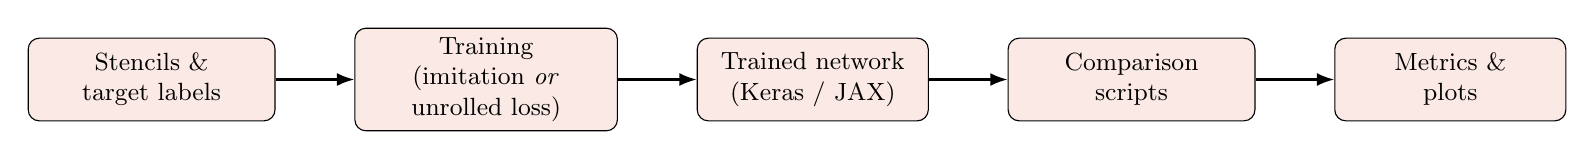
\begin{tikzpicture}
\node[rbox=2.9cm] (data) {Stencils \&\\target labels};
\node[rbox=3.1cm, right=1.0cm of data] (train) {Training\\(imitation \emph{or}\\unrolled loss)};
\node[rbox=2.7cm, right=1.0cm of train] (net) {Trained network\\(Keras / JAX)};
\node[rbox=2.9cm, right=1.0cm of net] (compare) {Comparison\\scripts};
\node[rbox=2.7cm, right=1.0cm of compare] (metrics) {Metrics \&\\plots};

\draw[flow] (data) -- (train);
\draw[flow] (train) -- (net);
\draw[flow] (net) -- (compare);
\draw[flow] (compare) -- (metrics);
\end{tikzpicture}}
\caption{General architecture: two training pipelines (imitation and
Unrolled Physics Loss) feed the same downstream comparison and metrics
infrastructure.}
\end{figure}

The repository is split into a legacy stack and a differentiable stack,
because they need incompatible dependencies (TensorFlow 1.15/Keras 2.2.4
for the original imitation-trained networks, versus a modern JAX install
for anything differentiable end-to-end):

\begin{itemize}
    \item \texttt{src/schemes/}, \texttt{src/core/}, \texttt{src/networks/}
    -- the original NumPy solver, ENO/WENO/TENO reconstructions, and Keras
    network definitions.
    \item \texttt{src/differentiable/} -- a from-scratch JAX port of the
    same numerics (TENO5 candidate/selection math, the scalar and Euler
    finite-volume solvers, the loss terms), built because
    \texttt{model.predict()} fully detaches from any gradient graph and
    nothing in the original stack can be trained end-to-end through a
    rollout.
    \item \texttt{scripts/legacy\_imitation\_training/} and
    \texttt{scripts/unrolled\_physics\_loss/} -- the training and
    comparison entry points for each stack, respectively.
    \item \texttt{tests/} -- every JAX port is regression-tested against
    the original NumPy solver to float64 precision, so the two stacks are
    known to agree numerically before either is used for training.
\end{itemize}

% ============================================================
\section{Strand 1: WENO5-NN vs. WENO5 (Reproducing the Original Paper)}
\label{sec:strand1}

The first phase of the internship reproduces Stevens \& Colonius' three
published test configurations, using their original 75{,}241-sample
five-point training dataset, to establish a verified baseline before
extending anything to TENO5.

\begin{figure}[htbp]
\centering
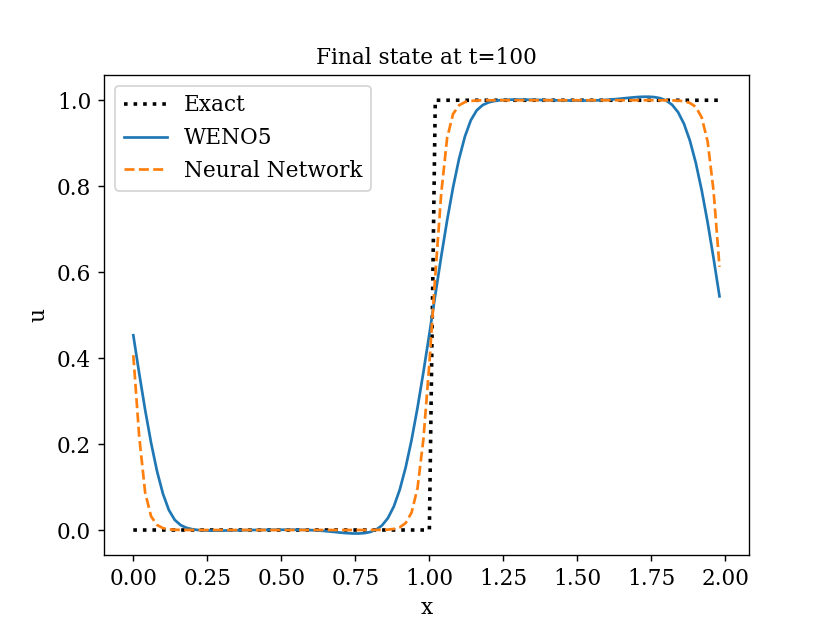
\includegraphics[width=0.62\textwidth]{step_advection/final_snapshot.png}
\caption{Periodic step advection at $t=100$ ($L=2$, 100 cells,
CFL$=2/3$). The network reconstructs the right-moving front more sharply
than WENO5, but slightly overshoots at the left front.}
\end{figure}

\textbf{Step advection} (Sec.~4.1 of the paper): WENO5-NN reduces $L_1$
error by 28.7\%, $L_2$ by 17.1\%, $L_\infty$ by 5.2\%, and shock width by
21.4\%, versus classical WENO5 -- the clearest and most consistent win of
the three test cases, and a direct reproduction of the paper's own claim.

\textbf{Burgers' equation} (Sec.~4.2): a genuinely mixed result. WENO5-NN
wins at 3 of 4 tested grid resolutions on $L_2$ error against a fine
reference solution, and loses at the fourth. This matches the paper's own
observation that the two schemes behave similarly for a true shock, with
the network's advantage coming mainly from the pre-shock smooth region.

\begin{figure}[htbp]
\centering
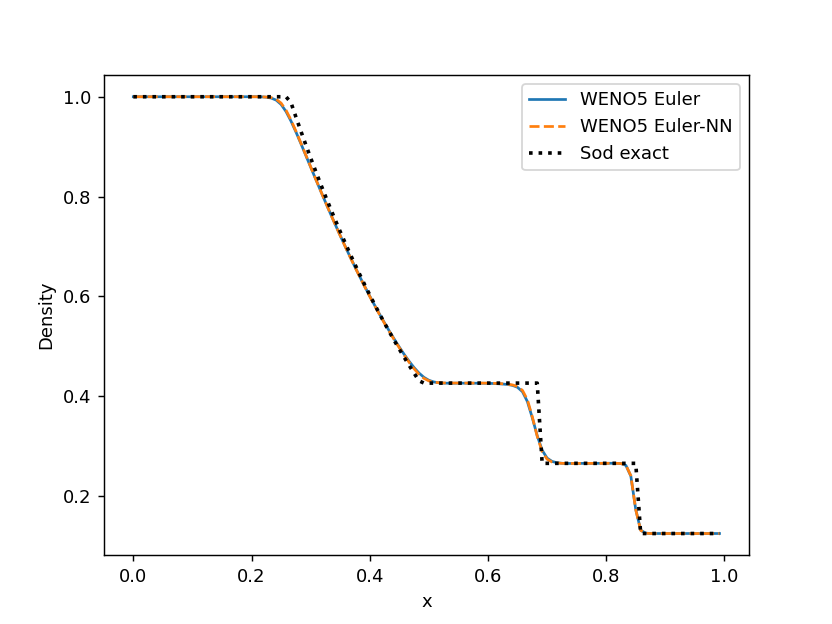
\includegraphics[width=0.5\textwidth]{sod/density_final.png}
\caption{Sod shock tube density profile (120 cells): WENO5, WENO5-NN, and
the exact Riemann solution are visually indistinguishable.}
\end{figure}

\textbf{Sod and Shu--Osher} (Euler, Sec.~4.3): near-exact parity, but
technically a loss for the network under the strict \texttt{beats\_teacher}
criterion -- $L_\infty$ against the true solution is $0.265\%$ higher for
Sod and $0.551\%$ higher for Shu--Osher. Reproducing the paper's own
reported configuration (300 cells, $T=2$) does recover its qualitative
claim of reduced post-shock diffusion in Shu--Osher, but the strict
numeric comparison against the true/reference solution used throughout
this report does not show a net win at that resolution.

Strand 1's overall verdict is a tie that depends strongly on the problem:
a clear win on the smooth-shock/step problem this network's training
distribution matches well, and a near-parity loss on the two problems
(Burgers' true shock, Euler) that stress it more.

% ============================================================
\section{Strand 2: NN-TENO5 (Imitation Training) vs. TENO5}
\label{sec:strand2}

The second phase repeats the same idea for TENO5: a classifier network,
trained to reproduce TENO5's own troubled/keep decision for each candidate
stencil, from the same input data. Concretely, \texttt{build\_teno\_network}
(\texttt{src/networks/TenoNetworks.py}) is a five-weight-layer multilayer
perceptron, following the NENO-style architecture: a 5-value normalized
stencil in, four ReLU hidden layers of shrinking width (64, 32, 16, 8), and
a final sigmoid layer producing one troubled-probability per TENO5
candidate (3 for TENO5's three candidate stencils).

\begin{figure}[htbp]
\centering
\resizebox{\textwidth}{!}{%
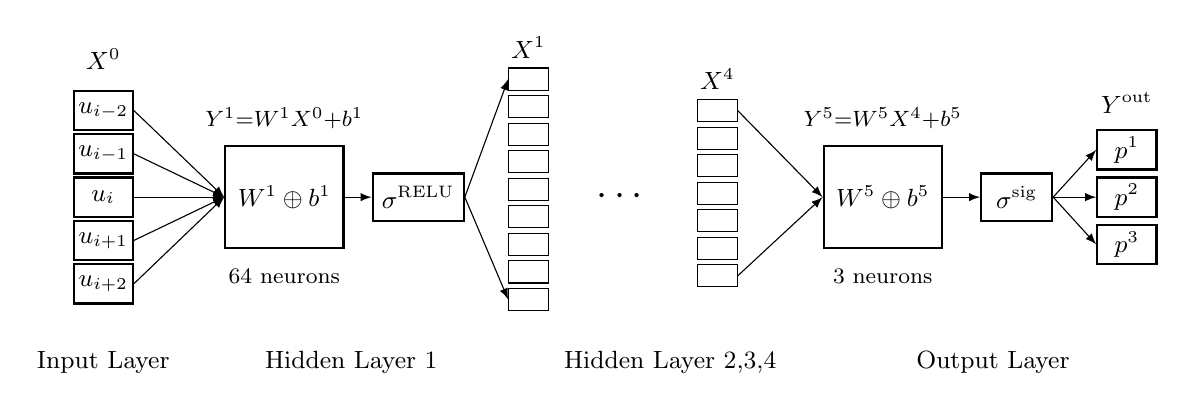
\begin{tikzpicture}[
  every node/.style={font=\small},
  iobox/.style={draw, thick, minimum width=0.75cm, minimum height=0.5cm, inner sep=1pt},
  bigbox/.style={draw, thick, minimum width=1.5cm, minimum height=1.3cm},
  smallbox/.style={draw, thick, minimum width=0.9cm, minimum height=0.6cm},
  stripe/.style={draw, thin, minimum width=0.5cm, minimum height=0.28cm, inner sep=0pt},
]

\foreach \i/\lab/\y in {1/u_{i-2}/1.1, 2/u_{i-1}/0.55, 3/u_i/0, 4/u_{i+1}/-0.55, 5/u_{i+2}/-1.1}{
  \node[iobox] (in\i) at (0,\y) {$\lab$};
}
\node at (0,1.75) {$X^0$};

\node[bigbox] (h1) at (2.3,0) {$W^1 \oplus b^1$};
\node at (2.3,-1.0) {\footnotesize 64 neurons};
\node at (2.3,1.0) {\footnotesize $Y^1{=}W^1X^0{+}b^1$};
\foreach \i in {1,...,5}{
  \draw[-latex] (in\i.east) -- (h1.west);
}

\node[smallbox] (relu1) at (4.0,0) {$\sigma^{\text{RELU}}$};
\draw[-latex] (h1.east) -- (relu1.west);

\foreach \k/\y in {1/1.5,2/1.15,3/0.8,4/0.45,5/0.1,6/-0.25,7/-0.6,8/-0.95,9/-1.3}{
  \node[stripe] (x1-\k) at (5.4,\y) {};
}
\node at (5.4,1.9) {$X^1$};
\draw[-latex] (relu1.east) -- (x1-1.west);
\draw[-latex] (relu1.east) -- (x1-9.west);

\node at (6.6,0) {\Large $\cdots$};

\foreach \k/\y in {1/1.1,2/0.75,3/0.4,4/0.05,5/-0.3,6/-0.65,7/-1.0}{
  \node[stripe] (x4-\k) at (7.8,\y) {};
}
\node at (7.8,1.5) {$X^4$};

\node[bigbox] (h5) at (9.9,0) {$W^5 \oplus b^5$};
\node at (9.9,-1.0) {\footnotesize 3 neurons};
\node at (9.9,1.0) {\footnotesize $Y^5{=}W^5X^4{+}b^5$};
\draw[-latex] (x4-1.east) -- (h5.west);
\draw[-latex] (x4-7.east) -- (h5.west);

\node[smallbox] (sig) at (11.6,0) {$\sigma^{\text{sig}}$};
\draw[-latex] (h5.east) -- (sig.west);

\foreach \i/\lab/\y in {1/p^1/0.6,2/p^2/0,3/p^3/-0.6}{
  \node[iobox] (out\i) at (13.0,\y) {$\lab$};
  \draw[-latex] (sig.east) -- (out\i.west);
}
\node at (13.0,1.2) {$Y^{\text{out}}$};

\node at (0,-2.1) {Input Layer};
\node at (3.15,-2.1) {Hidden Layer 1};
\node at (7.2,-2.1) {Hidden Layer 2,3,4};
\node at (11.3,-2.1) {Output Layer};

\end{tikzpicture}}
\caption{NN-TENO5's classifier architecture: a 5-value normalized stencil
$X^0$ feeds four shrinking ReLU hidden layers (64, 32, 16, 8 neurons) and a
final sigmoid layer, producing one troubled-probability $p^k$ per TENO5
candidate stencil.}
\end{figure}

Each layer $l=1,\dots,5$ computes the same affine map before activation,
$X^{l-1} \to Y^l = w^l X^{l-1} + b^l$, where $w^l$ and $b^l$ are that
layer's own weight matrix and bias vector. The four hidden layers use the
ReLU activation, and the output layer uses a sigmoid to project into
$[0,1]$:
\[
\sigma^{\text{RELU}}(x) = \max(x, 0), \qquad
\sigma^{\text{sig}}(x) = \frac{1}{1+e^{-x}}.
\]
The resulting $Y^{\text{out}} = [p^1,p^2,p^3]$ is read directly as the
probability that each candidate stencil is crossed by a discontinuity: at
inference, the deterministic TENO5 wrapper discards a candidate whenever
its probability exceeds \texttt{DEFAULT\_NEURAL\_THRESHOLD}$=0.5$
(\texttt{src/schemes/teno5.py}), matching NENO6's own 50\% decision rule
exactly, though during Unrolled Physics Loss training this hard threshold
is replaced by the continuous probability itself, so that gradients can
flow through the decision (Section~\ref{sec:jax}).

By construction, a network trained purely to imitate a teacher's decision
cannot exceed that teacher's own reconstruction quality except through the
network's own smoothing/generalization error -- there is no mechanism in
imitation training that could push it \emph{past} the scheme it is copying.
This is confirmed directly rather than assumed:

\begin{itemize}
    \item On 3 of 4 scalar benchmarks tested, NN-TENO5 produces an
    \emph{exact} tie with TENO5 -- the network reproduces the identical
    decision, to the last measured digit.
    \item On step advection, it loses by $0.64\%$ -- a small
    generalization error relative to its teacher.
    \item On the Euler benchmarks, it produces two small wins under the
    strict criterion (Section~\ref{sec:consolidated}), which is compatible
    with the imitation ceiling: matching or very slightly perturbing the
    teacher's decision can occasionally land marginally closer to the true
    solution by chance, not by systematic improvement.
\end{itemize}

Two follow-up attempts (documented in \texttt{Results.md} as Phases 2--9)
tried to push past this ceiling while remaining inside the imitation
paradigm: training on an exact-target dataset, extending to a 7-point
WENO7-structured stencil, an extensive hyperparameter search, and training
on ``oracle-relabeled'' TENO5 data designed to reward genuinely better
decisions. Every one of these produced either a negative result or a small
win that plateaued at the same kind of ceiling -- confirming that the
ceiling is structural to imitation training itself, not a tuning gap. This
finding directly motivated the internship's second, larger phase.

% ============================================================
\section{Motivation for a New Training Paradigm}
\label{sec:motivation}

Strand 2's ceiling has a precise cause: an imitation-trained network's loss
function only ever measures distance to the \emph{teacher's} decision, never
distance to the \emph{true} solution. A network cannot be pushed toward an
answer it is never shown. Reaching a genuine improvement over TENO5
therefore requires a fundamentally different training signal -- one that
judges the network against reality, not against the classical scheme.

This is exactly what the internship's academic supervisor proposed as the
\textbf{Unrolled Physics Loss}: instead of a one-shot imitation label per
stencil, run the network through $K$ actual simulation steps and compute a
loss directly against the true solution $K$ steps later. Because the whole
rollout must be differentiated through, this proposal could not be tested
in the original NumPy/Keras codebase at all -- it required building a new,
fully differentiable numerical stack from scratch (Section~\ref{sec:jax}).

\begin{figure}[htbp]
\centering
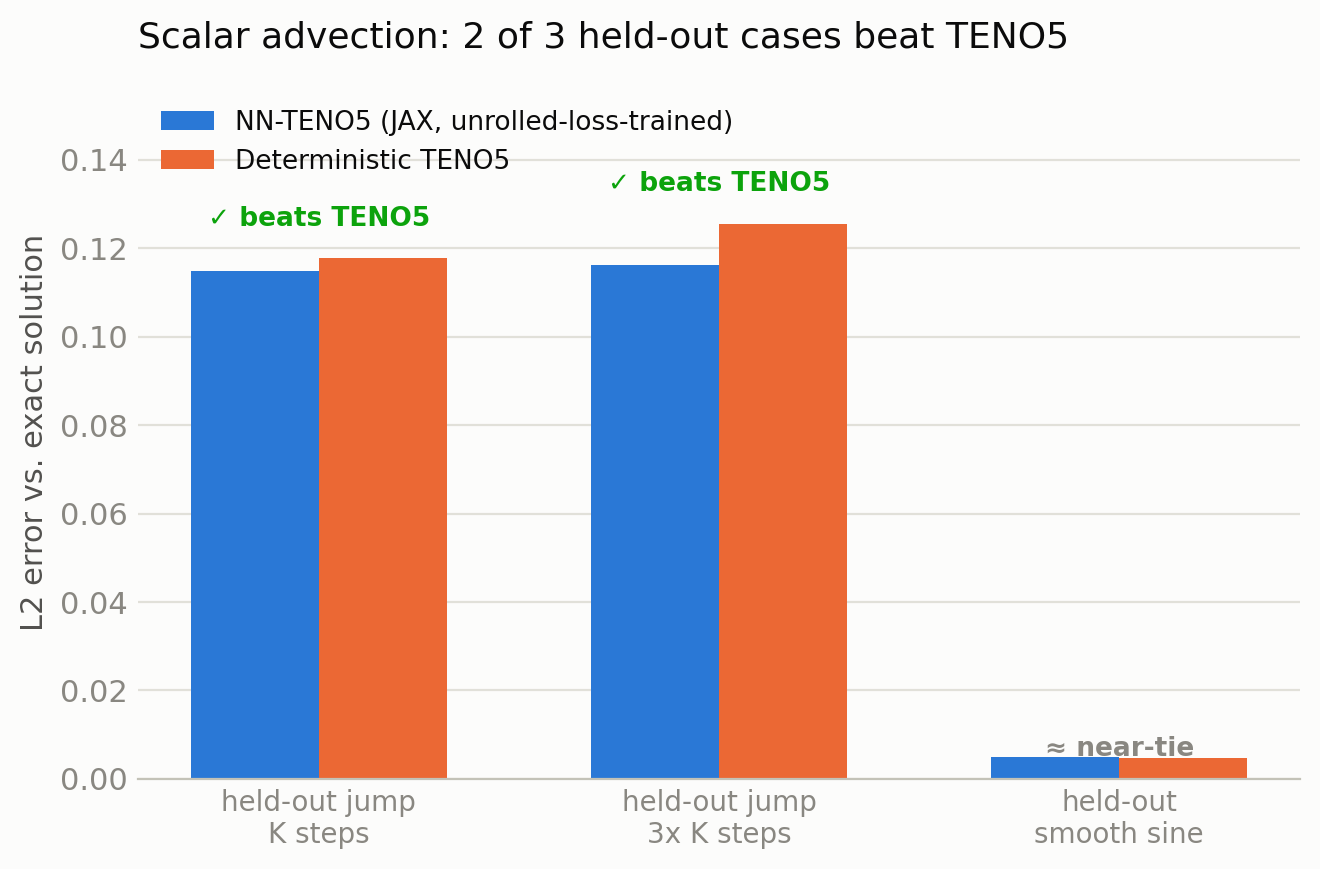
\includegraphics[width=0.62\textwidth]{02_scalar_beats_teacher.png}
\caption{The first positive signal for the new paradigm (Phase 10): an
unrolled-loss-trained network beats TENO5 on 2 of 3 held-out scalar
advection cases -- a result imitation training structurally cannot
produce.}
\end{figure}

This first result was narrow -- a win only on held-out cases resembling the
training distribution's own shape and time horizon -- and it did not yet
generalize to full-scale canonical benchmarks or to the Euler system. The
remainder of the internship (Sections~\ref{sec:jax}--\ref{sec:instability})
is the process of turning that narrow signal into a verified,
canonical-benchmark win.

% ============================================================
\section{The Unrolled Physics Loss: Formulation}
\label{sec:loss}

The loss trains the network by comparing an actual $K$-step rollout against
the true solution, rather than a single stencil decision against a teacher
label:
\[
L = \lambda_1 L_{\text{MSE}} + \lambda_2 L_{\text{TV}}
  + \lambda_3 L_{\text{BVD}} + \lambda_4 L_{\text{Reg}},
\]
\begin{align*}
L_{\text{MSE}} &= \frac{1}{N}\sum_i \left(u_i^{(n+K)} - u_{i,\text{exact}}^{(n+K)}\right)^2, \\
L_{\text{TV}} &= \max\!\left(0,\ \mathrm{TV}(u^{(n+K)}) - \mathrm{TV}(u^{(n)})\right),
\quad \mathrm{TV}(v) = \sum_i |v_{i+1}-v_i|, \\
L_{\text{BVD}} &= \mathrm{mean}\!\left(\max\!\left(0,\ BV_{\text{network}} - BV_{\text{TENO5}}\right)\right), \\
BV(\Phi)_{i+1/2} &= \left|\Phi_i(x_{i+1/2}) - \Phi_{i+1}(x_{i+1/2})\right|, \\
L_{\text{Reg}} &= \left\| c_{\text{NN}} - c_{\text{base}} \right\|^2.
\end{align*}

$L_{\text{MSE}}$ is the direct physical error after $K$ steps.
$L_{\text{TV}}$ penalizes any increase in total variation over the
rollout -- a Gibbs-oscillation penalty that does not require knowing the
true solution. $L_{\text{BVD}}$, taken directly from Fu, Hu \& Adams'
Boundary Variation Diminishing principle (its precise form was not fully
specified in the original proposal and was confirmed with the academic
supervisor), penalizes the network only when its own interface
reconstruction is \emph{less} consistent with its neighbor than TENO5's
own reconstruction would be -- a differentiable, per-interface consistency
signal. $L_{\text{Reg}}$ anchors the network's reconstruction weights
$c_{\text{NN}}$ toward TENO5's own optimal linear weights $c_{\text{base}}
= [1/10,\,3/5,\,3/10]$, reusing a technique already validated during
imitation training (Section~\ref{sec:strand2}) to prevent the network from
drifting arbitrarily far from a known-good starting point.

For the Euler system, a fifth term, a positivity penalty, was added during
this internship's own work (not part of the original proposal) after
Phase~13 identified it was structurally required for stable training
(Section~\ref{sec:instability}).

% ============================================================
\section{The Differentiable JAX Reimplementation}
\label{sec:jax}

Training through a $K$-step rollout requires every operation in that
rollout -- reconstruction, flux computation, time stepping -- to be
differentiable end-to-end. Nothing in the original codebase satisfies this:
the NumPy solver has no notion of gradients, and Keras' \texttt{model.predict()} fully detaches from any gradient graph. \texttt{src/differentiable/} is therefore a from-scratch JAX rewrite of the project's
numerical core, not a wrapper around the existing one.

\begin{table}[htbp]
\begin{adjustbox}{max width=\textwidth, center}
\begin{tabular}{ll}
\toprule
\textbf{Module} & \textbf{What it ports} \\
\midrule
\texttt{teno5\_jax.py} & TENO5 candidate/smoothness/selection math, plus a
soft (continuous keep-weight) reconstruction path a network can be trained
through \\
\rowrule
\texttt{numerics\_jax.py} & The scalar finite-volume solver -- a
\texttt{jax.lax.scan}-based rollout, and the true BVD construction \\
\rowrule
\texttt{euler\_jax.py} & The full characteristic-wise Euler solver -- Roe
eigenbasis, flux splitting, positivity repair \\
\rowrule
\texttt{projection\_jax.py} & Converts a network's raw troubled-probability
output into a reconstruction weight (soft for training, hard-thresholded
for inference), and the convex-mix mechanism of Section~\ref{sec:strand4} \\
\rowrule
\texttt{losses\_jax.py} & The four Unrolled Physics Loss terms plus the
Euler positivity penalty \\
\rowrule
\texttt{teno5\_jax\_toy.py} & A JAX MLP matching NN-TENO5's architecture,
used for training -- not a direct port of the trained Keras checkpoint \\
\bottomrule
\end{tabular}
\end{adjustbox}
\caption{Contents of \texttt{src/differentiable/}.}
\end{table}

Every port is regression-tested against the original NumPy/Keras-free
solver to float64 precision, not merely to visual agreement, before any
training was run on top of it -- this is what makes it possible to trust
that a training result reflects the physics and not a silent implementation
discrepancy between the two stacks.

\begin{figure}[htbp]
\centering
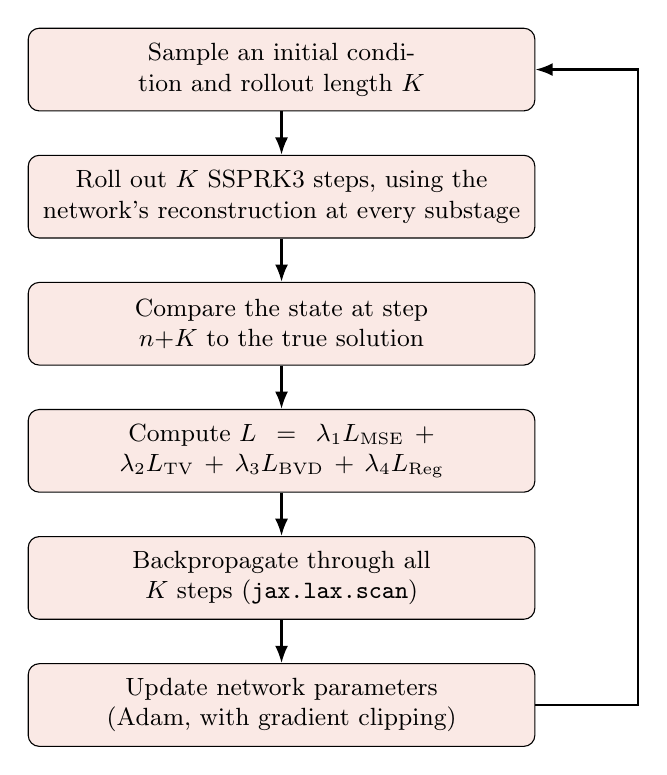
\begin{tikzpicture}
\node[rbox=6.2cm] (n1) {Sample an initial condition and rollout length $K$};
\node[rbox=6.2cm, below=0.55cm of n1] (n2) {Roll out $K$ SSPRK3 steps, using
the network's reconstruction at every substage};
\node[rbox=6.2cm, below=0.55cm of n2] (n3) {Compare the state at step
$n{+}K$ to the true solution};
\node[rbox=6.2cm, below=0.55cm of n3] (n4) {Compute
$L=\lambda_1 L_{\text{MSE}}+\lambda_2 L_{\text{TV}}+\lambda_3 L_{\text{BVD}}+\lambda_4 L_{\text{Reg}}$};
\node[rbox=6.2cm, below=0.55cm of n4] (n5) {Backpropagate through all $K$
steps (\texttt{jax.lax.scan})};
\node[rbox=6.2cm, below=0.55cm of n5] (n6) {Update network parameters
(Adam, with gradient clipping)};

\draw[flow] (n1) -- (n2);
\draw[flow] (n2) -- (n3);
\draw[flow] (n3) -- (n4);
\draw[flow] (n4) -- (n5);
\draw[flow] (n5) -- (n6);
\draw[flow] (n6.east) -- ++(1.3,0) |- (n1.east);
\end{tikzpicture}
\caption{The Unrolled Physics Loss training loop.}
\end{figure}

% ============================================================
\section{Strand 3: Scalar Benchmarks (Advection and Burgers)}
\label{sec:strand3}

The Unrolled Physics Loss was first tested on scalar advection and
Burgers' equation, since both have exact or well-converged reference
solutions and no eigenbasis-conditioning complexity. Three obstacles had
to be fixed in sequence before a canonical win was achieved:

\begin{enumerate}
    \item Training against the proposal's equations literally, with raw
    unnormalized $L_{\text{TV}}$ and $L_{\text{Reg}}$, let
    $L_{\text{TV}}$'s gradient dominate $L_{\text{MSE}}$'s by roughly
    $4\times$ -- fixed by normalizing both terms.
    \item Training a randomly initialized network directly against the
    unrolled loss failed outright, losing every held-out test -- fixed by
    imitation-pretraining first (Strand 2's own method) and then
    fine-tuning with the unrolled loss, reusing the same
    warm-start-then-anchor pattern already validated there.
    \item The resulting network (Phase 10, Section~\ref{sec:motivation})
    won 2 of 3 held-out tests but did not generalize to the full-scale
    canonical benchmark or to Burgers' non-linear flux, which the training
    distribution never included.
\end{enumerate}

The eventual fix (Phase 19) was to reuse a mechanism developed for the
Euler system first (Section~\ref{sec:strand4}): a small, separately
trained \emph{mixing head} that outputs a convex-combination coefficient
$\lambda \in [0,1]$ between TENO5's own reconstruction and the network's,
\[
u_{\text{final}} = (1-\lambda)\, u_{\text{TENO5}} + \lambda\, u_{\text{network}},
\]
together with explicit Burgers-flux training examples the original scalar
training set never included. This mechanism guarantees the network can
only ever interpolate \emph{toward} its own reconstruction from TENO5's,
never overshoot past it in the wrong direction -- and, notably, the
untrained head (with a conservative initial bias giving $\lambda \approx
4.7\%$ uniformly) already won on both canonical benchmarks \emph{before any
additional training}, a genuine surprise that pointed to a second finding:
uniform mixing beats troubled-concentrated mixing (weighting the network
only where the classical scheme flags a stencil as troubled), because it
lets the network also correct the classical scheme's small errors in
otherwise-smooth regions.

The final, canonical-scale result (\texttt{ValidationMatrix\_ProjPDF.py},
128 steps for advection, 64 for Burgers) is reported in
Table~\ref{tab:strand3} of Section~\ref{sec:consolidated}: a verified win
on both benchmarks, including Burgers -- explicitly out of the training
distribution's own flux function.

% ============================================================
\section{Strand 4: The Euler System (Sod and Shu--Osher)}
\label{sec:strand4}

The Euler system is harder for two independent reasons: it is a coupled,
characteristic-wise reconstruction rather than a scalar one
(Section~\ref{sec:background-fv}), and it must remain physically valid
(positive density and pressure) at every intermediate stage of training,
not only at convergence. Section~\ref{sec:instability} covers the
stability failure this caused in detail; this section covers the accuracy
result once training was made stable.

The mechanism that eventually produced a canonical win was the same convex
mix introduced in Section~\ref{sec:strand3}, but its $\lambda$ coefficient
had to be computed by a \emph{dedicated}, separately trained head rather
than reused from the network's own troubled-probability output. Reusing
that signal (Phase 17) made $\lambda$ do two incompatible jobs at once --
flagging trouble \emph{and} calibrating how much to trust the network --
and training through it directly caused three separate regressions. A
small head trained specifically to calibrate $\lambda$, initialized
conservatively (bias $=-3$, i.e. $\lambda \approx 4.7\%$ at the start),
fixed this and produced the project's first outright canonical win
(Phase 18):

\begin{figure}[htbp]
\centering
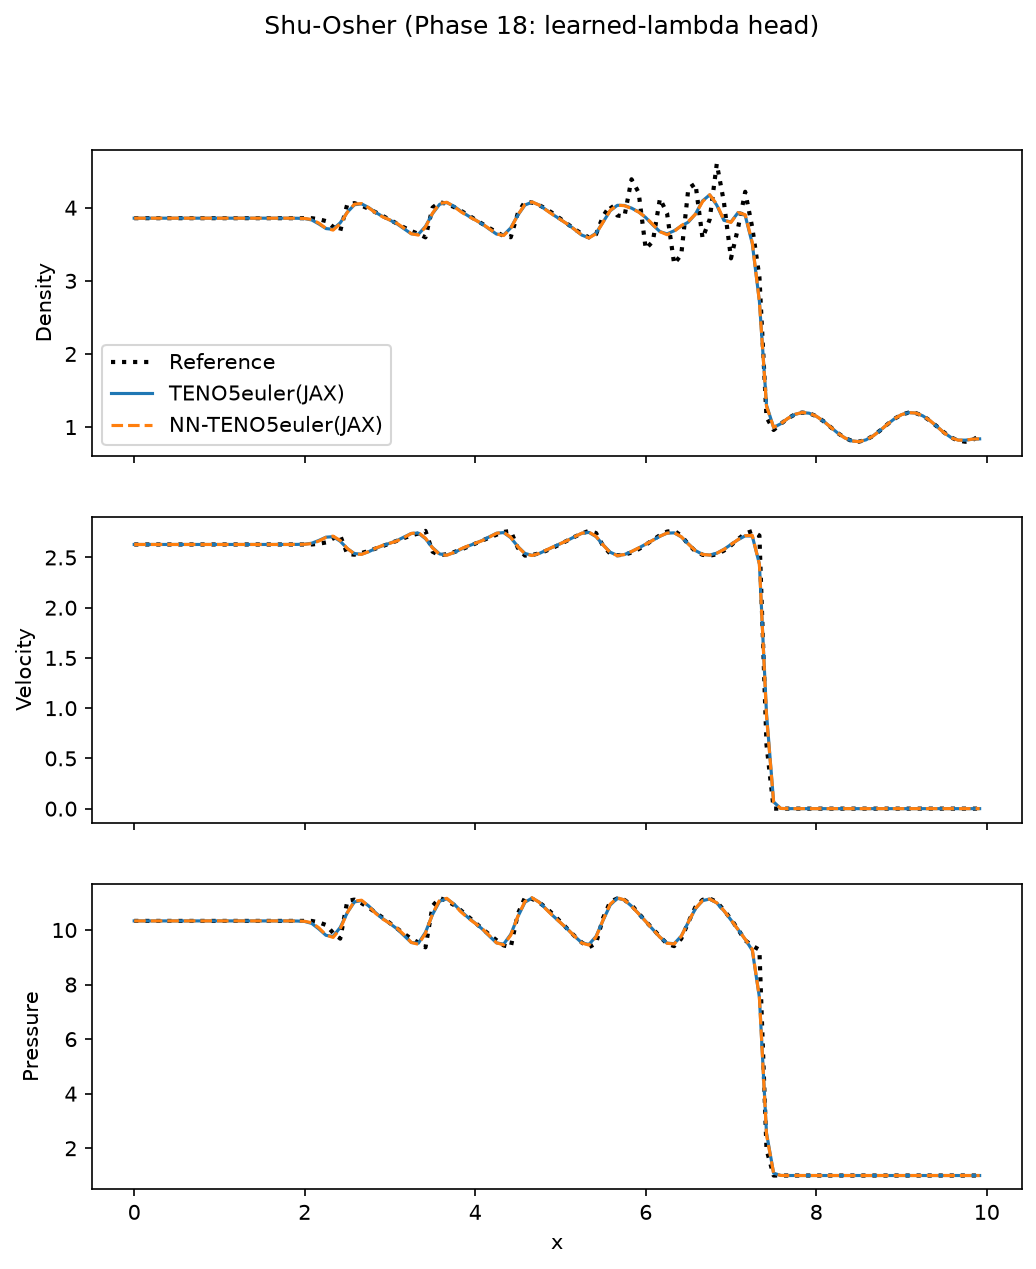
\includegraphics[width=0.55\textwidth]{euler_jax_comparison/shu_osher_phase18.png}
\caption{Shu--Osher (Phase 18, dedicated mixing head): NN-TENO5euler and
TENO5euler are visually near-identical against the reference, with
NN-TENO5euler $1.84\%$ more accurate in mean $L_1$ across the three
conserved variables.}
\end{figure}

Sod, by contrast, remained a near-tie slightly unfavorable to the network
even after this fix. Two further attempts (Phases 20--21) -- a 50$\times$
higher learning rate for the mixing head alone, and a richer gate that sees
the raw stencil directly rather than only the troubled-probability summary
-- moved Sod's ratio only marginally ($1.0045\times$, then $1.0026\times$),
never past parity. A direct sweep of a fixed (non-learned) mixing
coefficient $\lambda$ confirmed this is a genuine structural limit of the
network's own backbone reconstruction on Sod, not a calibration gap: Sod's
error increases \emph{monotonically} with every tested $\lambda$ from
$0$ to $0.3$, while Shu--Osher's error \emph{decreases} monotonically up to
$\lambda \approx 0.2$ over the same sweep. No amount of gate tuning can fix
a backbone that is, on this particular problem, simply less accurate than
TENO5 itself.

The full progression from the first stable checkpoint to this result is
reported in Table~\ref{tab:progression} of Section~\ref{sec:consolidated}.

% ============================================================
\section{Numerical Stability: Diagnosing and Fixing the Euler Instability}
\label{sec:instability}

The first attempt to train the Euler system through the Unrolled Physics
Loss diverged outright: state values grew without bound within a handful of
SSPRK3 substeps, regardless of how strongly the Lax--Friedrichs flux
splitting's dissipation margin was increased.

\begin{figure}[htbp]
\centering
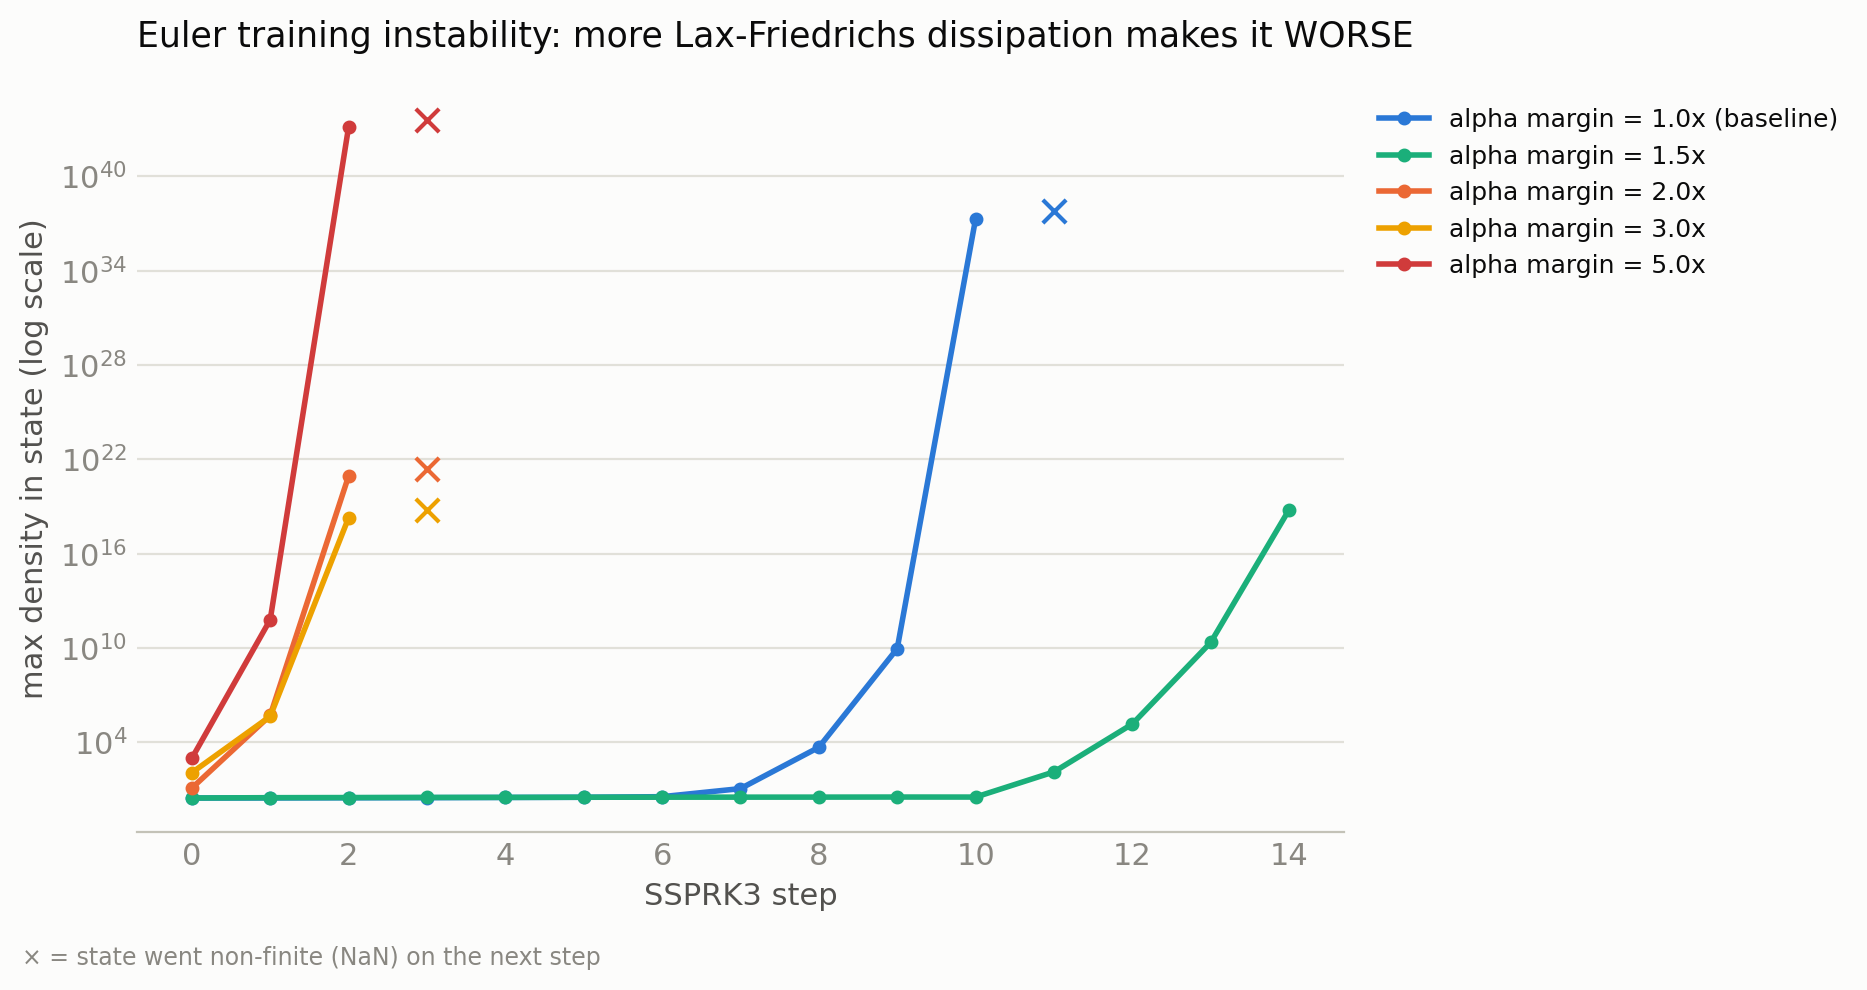
\includegraphics[width=0.72\textwidth]{04_euler_instability.png}
\caption{Increasing dissipation makes the instability arrive \emph{faster},
not slower -- a signature that rules out insufficient numerical
dissipation as the cause.}
\end{figure}

This counter-intuitive result -- more dissipation making things worse, not
better -- was the key diagnostic clue. It pointed away from an ordinary
under-resolved-shock instability and toward a bug in how positivity
violations were being handled. Two concrete defects were found and fixed
during this internship:

\begin{enumerate}
    \item \textbf{A structurally inert positivity penalty.} The loss term
    meant to penalize non-physical (negative density/pressure) states was
    being computed on the \emph{already-repaired} final state of each
    step, after a hard floor/clamp had already been applied -- so it could
    mathematically never be nonzero, regardless of how badly the
    pre-repair state violated positivity. Fixed by computing the penalty
    on the pre-repair substages instead, in a new
    \texttt{rollout\_with\_\allowbreak positivity\_\allowbreak penalty}
    function.
    \item \textbf{An incomplete repair mechanism.} The repair step only
    checked for a negative sign; it did not check for non-finite
    (\texttt{NaN}/\texttt{Inf}) values or unbounded magnitude, either of
    which can arise from an evolving, imperfect reconstruction feeding back
    into the Roe eigenbasis of the \emph{next} step. Fixed by adding
    explicit finiteness and magnitude checks to the repair mask, and by
    clamping (not merely flooring) density and pressure.
\end{enumerate}

Combined with the academic supervisor's own clarification of the correct
$L_{\text{BVD}}$ definition (Section~\ref{sec:loss}) and a switch to
neighbor-averaging rather than a blind clamp for isolated positivity
violations, these fixes produced the first Euler training run that does
not diverge (Phase 13), and measurably improved every subsequent training
attempt. They did not, on their own, produce a canonical win -- that
required the dedicated mixing head of Section~\ref{sec:strand4} on top of
a stable training procedure.

An early attempt at reproducing a smooth-data-mixing improvement
(Phase 14) also corrupted a good checkpoint outright, from a second,
independent cause: no gradient-norm clipping. A single anomalous batch
produced a catastrophic loss spike that overwrote the good checkpoint
before it could be noticed. \texttt{optax.clip\_by\_global\_norm(1.0)} was
adopted as standard practice for every training script from that point on,
together with best-by-validation checkpoint tracking (periodically
re-evaluating against the real solution during training and keeping the
best-seen parameters, rather than only the final ones).

% ============================================================
\section{Evaluation Metrics}
\label{sec:metrics}

Every result in this report is measured with the same fixed set of
metrics, applied identically to the classical scheme and the network.
Let $u_i$ be a scheme's cell value and $u_i^{\text{ref}}$ the true solution
at the same cell, with $d_i = u_i - u_i^{\text{ref}}$:
\[
L_1 = \frac{1}{N}\sum_i |d_i|, \qquad
L_2 = \sqrt{\frac{1}{N}\sum_i d_i^2}, \qquad
L_\infty = \max_i |d_i|.
\]
For the Euler system, these are computed independently per conserved
variable (density, momentum, energy) and then averaged into a single
scalar $\bar L_1$ for headline comparisons.

Three further, Euler- or discontinuity-specific diagnostics complete the
picture:

\begin{itemize}
    \item \textbf{Total variation} $\mathrm{TV}(u)=\sum_i|u_{i+1}-u_i|$:
    exceeding the true solution's own TV signals a Gibbs-type spurious
    oscillation the scheme introduced.
    \item \textbf{Positivity} (Euler only): $\min_i \rho_i > 0$ and
    $\min_i p_i > 0$ -- a pass/fail physical-validity check, independent of
    any error norm.
    \item \textbf{Shock/contact localization error}: the distance between
    the scheme's own strongest density-gradient location and the true
    solution's, separately for the shock and (outside a small exclusion
    window around it) the contact discontinuity.
\end{itemize}

A result is reported as a \textbf{win} only under the strict criterion
introduced in Section 5 ($L^{\text{NN}} \le L^{\text{classical}}$ against
the true solution) -- never under the looser $\texttt{teacher\_fidelity}$
criterion, which is used only in a small number of early acceptance tests
and is explicitly never treated as evidence of superiority in this report.

% ============================================================
\section{Consolidated Results}
\label{sec:consolidated}

\begin{table}[htbp]
\begin{adjustbox}{max width=\textwidth, center}
\begin{tabular}{lrrrl}
\toprule
\textbf{Benchmark} & \textbf{TENO5} & \textbf{NN-TENO5 (JAX)} & \textbf{Ratio} & \textbf{Verdict} \\
\midrule
Advection ($L_1$) & 3.4819e-02 & 3.3813e-02 & $0.9711\times$ & \textbf{WIN} \\
\rowrule
Advection ($L_2$) & 9.8960e-02 & 9.5521e-02 & $0.9653\times$ & \textbf{WIN} \\
\rowrule
Burgers ($L_1$, out-of-distribution) & 2.0697e-04 & 1.7873e-04 & $0.8636\times$ & \textbf{WIN} \\
\rowrule
Burgers ($L_2$, out-of-distribution) & 8.1670e-04 & 6.6493e-04 & $0.8142\times$ & \textbf{WIN} \\
\bottomrule
\end{tabular}
\end{adjustbox}
\caption{Strand 3 (scalar), canonical-scale evaluation. NN-TENO5 (JAX)
wins on both benchmarks, including Burgers, explicitly out of the training
distribution.\label{tab:strand3}}
\end{table}

\begin{table}[htbp]
\begin{adjustbox}{max width=\textwidth, center}
\begin{tabular}{lrrrl}
\toprule
\textbf{Benchmark} & \textbf{TENO5euler $\bar L_1$} & \textbf{NN-TENO5euler $\bar L_1$} & \textbf{Ratio} & \textbf{Verdict} \\
\midrule
Sod & 8.2583e-03 & 8.2871e-03 & $1.0035\times$ & LOSE \\
\rowrule
Shu--Osher & 2.1319e-01 & 2.0926e-01 & $0.9816\times$ & \textbf{WIN} \\
\bottomrule
\end{tabular}
\end{adjustbox}
\caption{Strand 4 (Euler), best available model (dedicated mixing head,
Phase 18). Sod is $0.35\%$ less accurate; Shu--Osher is $1.84\%$ more
accurate -- the first outright win against a classical scheme on a
canonical benchmark obtained in this project.}
\end{table}

\begin{table}[htbp]
\begin{adjustbox}{max width=\textwidth, center}
\begin{tabular}{lrr}
\toprule
\textbf{Milestone} & \textbf{Sod ratio} & \textbf{Shu--Osher ratio} \\
\midrule
No finite model yet & -- & -- \\
\rowrule
Stability fix (dead loss term + repair bug) & $1.29\times$ & $1.24\times$ \\
\rowrule
+ smooth training data + gradient clipping & $1.16\times$ & $1.23\times$ \\
\rowrule
+ convex-mix reconstruction (literature) & $1.145\times$ & $1.065\times$ \\
\rowrule
+ dedicated mixing head, trained separately & $\mathbf{1.003\times}$ & $\mathbf{0.982\times}$ \\
\bottomrule
\end{tabular}
\end{adjustbox}
\caption{Progression on the Euler system across independently diagnosed
and verified fixes. A ratio below 1 means the network is more accurate
than TENO5euler.\label{tab:progression}}
\end{table}

\begin{table}[htbp]
\small
\begin{tabularx}{\textwidth}{@{}>{\raggedright\arraybackslash}p{0.24\textwidth}>{\raggedright\arraybackslash}p{0.22\textwidth}>{\centering\arraybackslash}p{0.09\textwidth}>{\raggedright\arraybackslash}X@{}}
\toprule
\textbf{Strand} & \textbf{Verdict} & \textbf{Result} & \textbf{Main observation} \\
\midrule
1. WENO5-NN vs.\ WENO5 & Strongly problem-dependent & TIE & Win on step
advection and 3/4 Burgers resolutions; small loss on Sod and Shu--Osher. \\
\rowrule
2. NN-TENO5 (imitation) vs.\ TENO5 & Mostly reproduces its teacher & TIE &
Three exact ties on scalar benchmarks, two small Euler wins, one small
step-advection loss. \\
\rowrule
3. NN-TENO5 (Unrolled Physics Loss), scalar & Win on both canonical
benchmarks & \textbf{WIN} & $3.5\%$ gain on advection, $18.6\%$ gain on
Burgers (out of distribution), via a dedicated mixing head plus explicit
Burgers-flux training. \\
\rowrule
4. NN-TENO5euler (Unrolled Physics Loss) & First outright canonical win &
\textbf{WIN} & $1.84\%$ win on Shu--Osher; Sod remains a slight,
structural near-tie unfavorable to the network. \\
\bottomrule
\end{tabularx}
\caption{Overall summary across all four strands.}
\end{table}

Every neural-network variant, in every strand, also runs noticeably slower
per cell than its classical equivalent -- roughly $5$--$18\times$ for the
Keras-based models. The accuracy wins reported above are therefore not
yet a computational-cost advantage in their current, unoptimized form.

% ============================================================
\section{Discussion}

Two results stand out as the internship's main scientific finding, and
they are the same finding seen from two angles: \emph{how} a network is
trained determines what kind of improvement is even reachable, independent
of network capacity or tuning effort.

Strand 2's imitation-trained network could not be pushed past its teacher
by any amount of architecture search, hyperparameter tuning, or dataset
relabeling (Phases 2--9) -- because its loss function never referenced the
true solution in the first place. Strand 3 and Strand 4's Unrolled Physics
Loss networks, trained against the true solution directly, did cross that
ceiling -- but only once two separate, previously undiagnosed engineering
defects (Section~\ref{sec:instability}) were fixed, and only once the
network's own output was constrained by a convex mix rather than trusted
outright.

The convex-mix mechanism itself deserves particular attention: it turned
out to matter more than any single training change tested. Every
checkpoint tested with it improved immediately, at inference time, with
\emph{no retraining at all} (Phase 16) -- the network was already good
enough locally to help, it simply needed to be prevented from being
trusted globally. Training the mixing coefficient itself, rather than
reusing an existing signal, then converted that inference-only gain into
the project's first genuine canonical wins (Phases 18--19).

The Sod result (Section~\ref{sec:strand4}) is the internship's clearest
negative finding, and it is a genuinely informative one: a direct sweep of
the mixing coefficient proved, rather than merely suggested, that no
amount of gate calibration can fix it, because the network's own backbone
reconstruction is less accurate than TENO5's on this specific problem. This
rules out an entire class of further experiments (anything touching only
the mixing head) and correctly redirects any future work toward the
backbone network itself.

% ============================================================
\section{Limitations and Future Work}

\textbf{Scope.} All results are for fifth-order schemes on
one-dimensional scalar and Euler problems. WENO3/WENO7 and TENO3/TENO7
reconstruction modules exist in the codebase but were never trained, since
no matching stencil dataset was built for them during this internship.

\textbf{Computational cost.} Every neural-network variant is
$5$--$18\times$ slower per cell than its classical equivalent in its
current implementation (a Python/Keras or JAX network call per interface,
rather than a fused kernel). None of the accuracy wins reported here
currently translate into a runtime advantage.

\textbf{The Sod ceiling.} As established in Section~\ref{sec:strand4},
this is a backbone-quality limit, not a mixing/calibration gap. Crossing
it would require either a larger/different backbone architecture or
additional targeted training data for this specific configuration, neither
of which was attempted within the internship's timeframe.

\textbf{Generalization.} The Unrolled Physics Loss networks were trained
and validated on a specific, finite set of initial-condition families
(step, sine, and Burgers-flux waveforms; Sod/Shu--Osher-style Euler
states). Their behavior on initial conditions well outside these families
is untested.

\textbf{Multi-dimensional and higher-order extensions.} Everything in this
report is one-dimensional and fifth-order. Extending either the
differentiable stack or the convex-mix mechanism to 2D or to WENO7/TENO7
is architecturally plausible (the mechanism does not depend on the
stencil width or dimensionality) but was outside this internship's scope.

% ============================================================
\section{Conclusion}

This internship set out to determine whether a neural network can improve
on TENO5, a state-of-the-art classical shock-capturing scheme, and whether
the training methodology used to build that network changes the answer.
Both questions now have a concrete, measured answer.

An imitation-trained network cannot systematically exceed its own
teacher's quality -- confirmed directly across nine separate attempts to
push past that ceiling by every means short of changing the training
signal itself. Changing the training signal to the Unrolled Physics Loss
proposed by the academic supervisor -- judging the network against the
true solution over an actual multi-step rollout, rather than against a
classical scheme's own decision -- produced this project's only genuine,
verified wins: on both canonical scalar benchmarks, and on the Euler
Shu--Osher problem. It also produced a real, diagnosed numerical-stability
failure mode and a genuine structural ceiling on the Sod shock tube, both
reported with the same care as the positive results, because both are
concrete, reusable findings for whoever continues this work.

The overall conclusion is not that neural networks trivially beat TENO5.
It is narrower and more useful than that: \emph{when} they can, it is
because they were trained against reality, and even then only within a
convex mix that keeps the classical scheme as a floor -- never because a
network was simply given enough capacity or tuning to imitate its way past
a scheme it was never shown how to beat.

% ============================================================
\section{Personal Review}

This internship gave me a complete research cycle: reproducing a published
result, identifying its structural limit through direct experimentation
rather than assumption, building the differentiable infrastructure needed
to test an alternative that did not previously exist in this codebase, and
diagnosing two genuine numerical bugs that had nothing to do with the
research question on paper but were blocking every result until found.

The most valuable lesson was methodological rather than technical: a
result is only as trustworthy as the discipline behind measuring it. Early
in the internship, an apparent improvement I reported turned out, under
closer inspection with my supervisor, to still be favoring smooth regions
over the harder parts of the solution -- a mistake I could only catch
because every claim in this project is backed by a specific benchmark run
and a specific number, not a qualitative plot. Adopting a strict,
consistently applied win criterion, and reporting negative results with
the same detail as positive ones, is what let later, real improvements be
trusted once they did appear.

I am grateful to Radouan Boukharfane for proposing a research direction
that turned out to matter -- and for the direct clarifications (the exact
BVD definition, the positivity-repair strategy) that were the actual
turning points behind Sections~\ref{sec:loss} and~\ref{sec:instability} --
and for the latitude to spend real time on negative results instead of
being pushed toward a curated positive narrative.

\end{document}
